% posets.tex
% updated January 11, 2012

\chapter{Partially Ordered Sets}\label{ch:posets}

Alice was surfing the web and found a site listing top movies, grouped
by categories (comedy, drama, family, etc) as well as by the decade in 
which they were released.  Alice was intrigued by the critic's choices
and his rankings, especially for the top seven dramas from the 1990's.
Alice agreed with the critic's choices as a group but not the
specific rankings.  She wrote the critic's rankings on the board
and just to the right, she gave her own rankings, all the time
insisting that she was certainly correct in her opinions.


\begin{center}
\begin{minipage}{.45\textwidth}
\noindent
\textbf{Movie Critic's Ranking}

\begin{enumerate}
\item Saving Private Ryan 
\item Life is Beautiful 
\item Forrest Gump
\item Braveheart
\item Good Will Hunting
\item Titanic
\item Jurassic Park
\end{enumerate}
\end{minipage}
\begin{minipage}{.45\textwidth}
\noindent
\textbf{Alice's Ranking}

\begin{enumerate}
\item Life is Beautiful 
\item Saving Private Ryan 
\item Good Will Hunting
\item Titanic
\item Braveheart
\item Forrest Gump
\item Jurassic Park
\end{enumerate}
\end{minipage}
\end{center}

Dave studied the two rankings and listened carefully to Alice's rationale
(which he felt was a bit over the top), but eventually, he held up the following
diagram and offered it as a statement of those comparisons on which both Alice
and the movie critic were in agreement. 

\begin{figure}
\begin{center}
\includegraphics*[scale=.4]{posets-figs/movies.pdf}
\caption{Top Movies from the 90's}
\label{fig:movies}
\end{center}
\end{figure}

\begin{remark}
Do you see how Dave made up this diagram?  Add your own rankings of these
seven films and then draw the diagram that Dave would produce as a statement
about the comparisons on which you, Alice and the movie critic were in agreement.
\end{remark}

More generally, when humans are asked to express preferences among 
a set of options, they often report that establishing a totally ranked list 
is difficult if not impossible.  Instead, they prefer to report a partial 
order---where comparisons are made between certain pairs of options but not 
between others.  In this chapter, we
make these observations more concrete by introducing the concept of 
a partially ordered set.  Elementary examples include (1)~a family of sets which is 
partially ordered by inclusion and (2)~a set of positive integers which is
partially ordered by division.  From an applications standpoint, a
complex construction job typically involves a large number of projects
for which there is a notion of precedence between some but not all pairs.
Also, computer file systems are modeled by trees which become partially 
ordered sets whenever links are added.

\section{Basic Notation and Terminology}\label{s:posets:intro}

A \textit{partially ordered set} or \textit{poset} $\bfP$ is a pair
$(X,P)$ where $X$ is a set and $P$ is a reflexive, antisymmetric, and
transitive binary relation on $X$. (Refer to \autoref{s:order} for a
refresher of what these properties are if you need to.) We call $X$
the \textit{ground set} while $P$ is a \textit{partial order} on
$X$. Elements of the ground set $X$ are also called \textit{points},
and the poset $\bfP$ is \textit{finite} if its ground set $X$ is a
finite set.

\begin{example}\label{exa:binaryrel}
Let $X=\{a,b,c,d,e,f\}$ and consider the following binary relations
on $X$.
\begin{enumerate}
\item $R_1=\{(a,a),(b,b),(c,c),(d,d),(e,e),(f,f),(a,b),(a,c),(e,f)\}$.
\item $R_2=\{(a,a),(b,b),(c,c),(d,d),(e,e),(f,f),(d,b),(d,e),(b,a),(e,a),$\\
 $(d,a),(d,e),(c,f)\}$.
\item $R_3=\{(a,a),(b,b),(c,c),(d,d),(e,e),(f,f),(a,c),(a,e),(a,f),(b,c),$\\
 $(b,d),(b,e),(b,f),(d,e),(d,f),(e,f)\}$.
\item $R_4=\{(a,a),(b,b),(c,c),(d,d),(e,e),(f,f),(d,b),(b,a),(e,a),(c,f)\}$.
\item $R_5=\{(a,a),(c,c),(d,d),(e,e),(a,e),(c,a),(c,e),(d,e)\}$.
\item $R_6=\{(a,a),(b,b),(c,c),(d,d),(e,e),(f,f),(d,f),(b,e),(c,a),(e,b)\}$.
\end{enumerate}
Then $R_1$, $R_2$ and $R_3$ are partial orders on $X$, so $\bfP_1=(X,R_1)$,
$\bfP_2=(X,R_2)$ and $\bfP_3=(X,R_3)$ are posets.  Several of the other examples
we will discuss in this chapter will use the poset $\bfP_3=(X,R_3)$.  

On the other hand, $R_4$, $R_5$ and $R_6$ are not partial orders on
$X$.  Note that $R_4$ is not transitive, as it contains $(d,b)$ and
$(b,a)$ but not $(d,a)$.  The relation $R_5$ is not reflexive, since
it doesn't contain $(b,b)$.  (Also, it also doesn't contain $(f,f)$,
but one shortcoming is enough.) Note that $R_5$ is a partial order on
$\{a,b,d,e\}$.  The relation $R_6$ is not antisymmetric, as it
contains both $(b,e)$ and $(e,b)$.
\end{example}

When $\PXP$ is a poset, it is common to write $x\le y$ in $P$ and
$y\ge x$ in $P$ as substitutes for $(x,y)\in P$. Of course, the notations $x<y$ in
$P$ and $y>x$ in $P$ mean $x\le y$ in $P$ and $x\ne y$.  When the
poset $\bfP$ remains fixed throughout a discussion, we will sometimes
abbreviate $x\le y$ in $P$ by just writing $x\le y$, etc.  When $x$
and $y$ are distinct points from $X$, we say $x$ is \textit{covered}
by $y$ in $P$\footnote{Reflecting the vagaries of the English
  language, mathematicians use the phrases: (1) $x$ is covered by $y$
  in $P$; (2)~$y$ covers $x$ in $P$; and (3)~$(x,y)$ is a cover in $P$
  interchangeably.}  when $x<y$ in $P$, and there is no point $z\in X$
for which $x<z$ an $z<y$ in $P$.  For example, in the poset
$\bfP_3=(X,R_3)$ from
\hyperref[exa:binaryrel]{Example~\ref*{exa:binaryrel}}, $d$ is covered
by $e$ and $c$ covers $b$. However, $a$ is not covered by $f$, since
$a<e<f$ in $R_3$.  We can then associate with the poset $\bfP$ a
\textit{cover graph} $\mathbf{G}$ whose vertex set is the ground set
$X$ of $\bfP$ with $xy$ an edge in $\mathbf{G}$ if and only if one of
$x$ and $y$ covers the other in $\bfP$.  Again, for the poset $\bfP_3$
from \hyperref[exa:binaryrel]{Example~\ref*{exa:binaryrel}}, we show
the cover graph on the left side of \autoref{fig:covergraphs}.
Actually, on the right side of this figure is just another drawing of
this same graph.

\begin{figure}
\begin{center}
\includegraphics*[scale=.4]{posets-figs/covergraphs.pdf}
\caption{Cover Graph}
\label{fig:covergraphs}
\end{center}
\end{figure}

It is convenient to illustrate a poset with a suitably drawn diagram
of the cover graph in the Euclidean plane.  We choose a standard
horizontal/vertical coordinate system in the plane and require that
the vertical coordinate of the point corresponding to $y$ be larger
than the vertical coordinate of the point corresponding to $x$
whenever $y$ covers $x$ in $P$. Each edge in the cover graph is
represented by a straight line segment which contains no point
corresponding to any element in the poset other than those associated
with its two end points.  Such diagrams are called \textit{Hasse
  diagrams} (\textit{poset diagrams, order diagrams}, or just
\textit{diagrams}).  Now it should be clear that the drawing on the
right side of \autoref{fig:covergraphs} is a diagram of the poset
$\bfP_3$ from \hyperref[exa:binaryrel]{Example~\ref*{exa:binaryrel}},
while the diagram on the left is not.

For posets of moderate size, diagrams are frequently used to define a poset---rather
than the explicit binary relation notation illustrated in \hyperref[exa:binaryrel]{Example~\ref*{exa:binaryrel}}.
In \autoref{fig:17ptposet}, we illustrate a poset $\PXP$ with ground set 
$X=[17]=\{1,2,\dots,17\}$.  It would take several lines of text to write out the
binary relation $P$, and somehow the diagram serves to give us a more tactile sense
of the properties of the poset. 

\begin{figure}
\begin{center}
\includegraphics*[scale=.4]{posets-figs/17ptposet.pdf}
\caption{A Poset on 17 Points}
\label{fig:17ptposet}
\end{center}
\end{figure}

\begin{remark}
Alice and Bob are talking about how you communicate with
a computer in working with posets.  Bob says that computers
have incredible graphics capabilities these days and that you
just give the computer a pdf scan of a diagram.  Alice says
that she doubts that anybody really does that.  Carlos says
that there are several effective strategies.  One way is to label 
the points with positive integers from $[n]$ where $n$ is the 
number of points in the ground set and then define a $0$--$1$
$n\times n$ matrix $A$ with entry $a(i,j)=1$ when $i\le j$ in $P$
and $a(i,j)=0$ otherwise.  Alternatively, you can just provide
for each element $i$ in the ground set a vector $U(x)$ listing all
elements which are greater than $x$ in $P$.  This vector can
be what computer scientists call a \textit{linked list}.
\end{remark}
 
\begin{example}\label{exa:construct}
There are several quite natural ways to construct posets.
\begin{enumerate}
\item A family $\mathcal{F}$ of sets is partially ordered by
inclusion, i.e., set $A\le B$ if and only if $A$ is a subset of
$B$.  
\item A set $X$ of positive integers is partially ordered by
division---without remainder, i.e., set $m\le n$ if and only if
$n\equiv 0\pmod{m}$.  
\item A set $X$ of $t$-tuples of real numbers is
partially ordered by the rule: \\
$(a_1,a_2,\dots,a_t)\le (b_1,b_2,\dots,b_t)$ if
and only if $a_i\le b_i$ in the natural order on $\reals$ for $i=1,2,\dots,t$.
\item When $L_1$, $L_2,\dots,L_k$ are linear orders on the same set
$X$, we can define a partial order $P$ on  $X$ by setting
$x\le y$ in $P$ if and only if $x\le y$ in $L_i$ for all $i=1,2,\dots,k$.
\end{enumerate}
We illustrate the first three constructions with the posets shown in 
\autoref{fig:constructposets}.  As is now clear, in the discussion at the 
very beginning of this chapter, Dave drew a diagram for the poset determined by 
the intersection of the linear orders given by Alice and the movie critic.
\end{example}

\begin{figure}
\begin{center}
\includegraphics*[scale=.4]{posets-figs/constructposets.pdf}
\caption{Constructing Posets}
\label{fig:constructposets}
\end{center}
\end{figure}

Distinct points $x$ and $y$ in a poset $\PXP$ are \textit{comparable}
if either $x<y$ in $P$ or $x>y$ in $P$; otherwise $x$ and $y$ are
\textit{incomparable}.  With a poset $\PXP$, we associate a 
\textit{comparability} graph ${\bfG}_1=(X,E_1)$ and an 
\textit{incomparability} graph ${\bfG}_2=(X,E_2)$. The edges in the 
comparability graph ${\bfG}_1$ consist of the comparable pairs and 
the edges in the incomparability graph are the incomparable pairs.  We 
illustrate these definitions in \autoref{fig:compincomp}
where we show the comparability graph and the incomparability graph
of the poset $\bfP_3$.

\begin{figure}
\begin{center}
\includegraphics*[scale=.4]{posets-figs/compincomp.pdf}
\caption{Comparability and Incommparability Graphs}
\label{fig:compincomp}
\end{center}
\end{figure}

A partial order $P$ is called a \textit{total} order (also, a 
\textit{linear} order) if for all $x,y\in X$, either $x\le y$ in $P$
or $y\le x$ in $P$.  For small finite sets, we can specify a linear
order by listing the elements from least to greatest.  For example,
$L=[b,c,d,a,f,g,e]$ is the linear order on the ground set $\{a,b,c,d,e,f,g\}$ with
$b<c<d<a<f<g<e$ in $L$.   

The set of real numbers comes equipped with a natural total order.  For example,
$1<7/5<\sqrt{2}<\pi$ in this order.  But in this chapter, we will be interested
primarily with partial orders that are \textit{not} linear orders.  Also, we note
that special care must be taken when discussing partial orders on ground sets
whose elements are real numbers.  For the poset shown in \autoref{fig:17ptposet}, note
that $14$ is less than $8$, while $3$ and $6$ are incomparable.
Best not to tell your parents that you've learned that under certain circumstances,
$14$ can be less than $8$ and that you may be able to say which of $3$ and $6$ is 
larger than the other.  The subtlety may be lost in the heated 
discussion certain to follow.

When $\PXP$ is a poset and $Y\subseteq X$, the binary relation
$Q=P\cap(Y\times Y)$ is a partial order on $Y$, and we call the
poset $(Y,Q)$ a \textit{subposet} of $\bfP$.  In \autoref{fig:subposet},
we show a subposet of the poset first presented in \autoref{fig:17ptposet}.

\begin{figure}
\begin{center}
\includegraphics*[scale=.4]{posets-figs/subposet.pdf}
\caption{A Subposet}
\label{fig:subposet}
\end{center}
\end{figure}

When $\PXP$ is a poset and $C$ is a subset of $X$,
we say that $C$ is a \textit{chain} if every distinct pair of points 
from $C$ is comparable in $P$.  When $P$ is a linear order, the entire ground 
set $X$ is a chain.  Dually, if $A$ is a subset of $X$, we say that
$A$ is an \textit{antichain} if every distinct pair of points from $A$ 
is incomparable in $P$.  Note that a one-element subset
is both a chain and an antichain.  Also, we consider the emptyset as
both a chain and an antichain.

The \textit{height} of a poset
$(X,P)$, denoted $\height(P)$, is the largest $h$ for which there exists
a chain of $h$ points in $P$.
Dually, the \textit{width} of a poset $\PXP$, denoted $\width(P)$, is the
largest $w$ for which there exists an antichain of $w$ points in
$P$. 

\begin{remark}
Given a poset $\PXP$, how hard is to determine its height and width?
Bob says that it is very easy.  For example, to find the width of a poset, just 
list all the subsets of $X$.  Delete those which are not antichains.
The answer is the size of the largest subset that remains.  He is quick
to assert that the same approach will work to find the height.
Alice groans at Bob's naivety and suggests that he should read
further in this chapter.
\end{remark}

\section{Additional Concepts for Posets}

We say $(X,P)$ and $(Y,Q)$ are \textit{isomorphic}, and write $(X,P)
\cong(Y,Q)$ if there exists a bijection (1--1 and
onto map) $f:X\to Y$ so that $x_1\le x_2$ in $P$ if and only if
$f(x_1)\le f(x_2)$ in $Q$. In this definition, the map $f$ is called an
\textit{isomorphism} from $\bfP$ to $\bfQ$.  In \autoref{fig:constructposets},
the first two posets are isomorphic.

\begin{remark}  Bob sees a pattern linking the first two posets
shown in \autoref{fig:constructposets} and asserts that any poset of one of these
two types is isomorphic to a poset of the other type.  Alice admits that Bob
is right---but even more is true.  The four constructions given in 
Example~\ref{exa:construct} are universal in the sense that \textit{every}
poset is isomorphic to a poset of each of the four types.  Do you see why? 
If you get stuck answering this, we will revisit the question at the
end of the chapter, and we will give you a hint.
\end{remark}

An isomorphism from $\bfP$ to 
$\bfP$ is called an \textit{automorphism} of $\bfP$. An isomorphism from 
$\bfP$ to a subposet of $\bfQ$ is called an \textit{embedding} of
$\bfP$ in $\bfQ$. In most settings, we will not distinguish between
isomorphic posets, and we will say that a poset $\PXP$ is \textit{contained}
in $\QYQ$ (also $\bfQ$ \textit{contains} $\bfP$) when there is an
embedding of $\bfP$ in $\bfQ$. Also, we will say that $\bfP$ \textit{excludes}
$\bfQ$ when no subposet of $\bfP$ is isomorphic to $\bfQ$, and we will 
frequently say $\bfP=\bfQ$ when $\bfP$ and $\bfQ$ are isomorphic.

With the notion of isomorphism, we are lead naturally to the notion of
an ``unlabelled'' posets, and in \autoref{f:unlabelled}, we show a
diagram for such a poset.

\begin{figure}[hb]
\begin{center}
\includegraphics*[scale=.4]{posets-figs/wttfig-5.pdf}
\caption{\label{f:unlabelled}An Unlabelled Partially Ordered Set}
\end{center}
\end{figure}

\begin{remark}
How hard is it to tell whether two posets are isomorphic?  Bob thinks
it's not too difficult.  Bob says that if you give him a bijection between
the ground sets, then he can quickly determine whether you have
established that the two posets are isomorphic.  Alice senses that
Bob is confusing the issue of testing whether two posets are isomorphic
with simply verifying that a particular bijection can be certified to
be an isomorphism.  The first problem seems much harder to her. Carlos says that he
thinks it's actually very hard and that in fact, no one knows whether there is
a good algorithm.  
\end{remark}

Note that the poset shown in \autoref{f:unlabelled} has the property
that there is only one maximal point.  Such a point is sometimes
called a \textit{one}, denoted not surprisingly as~$1$.  Also, there
is only one minimal point, and it is called a \textit{zero},
denoted~$0$.

The \textit{dual} of a partial order $P$ on a set $X$ is denoted by
$P^d$ and is defined by $P^d=\{(y,x):(x,y)\in P\}$. The \textit{dual}
of the poset $\PXP$ is denoted by $\bfP^d$ and is defined by
$\bfP^d=(X,P^d)$. A poset $\bfP$ is \textit{self-dual} if
$\bfP=\bfP^d$.

A poset $\PXP$ is \textit{connected} if its comparability graph is 
connected, i.e., for every $x,y\in X$ with
$x\ne y$, there is a finite sequence $x=x_0,x_1,\dots,x_n=y$ of points
from $X$ so that $x_i$ is comparable to $x_{i+1}$ in $P$ for
$i=0,1,2,\dots,n-1$. A subposet $(Y,P(Y))$ of $(X,P)$ is called a
\textit{component} of $\bfP$ if $(Y,P(Y))$ is connected and there is
no subset $Z\subseteq X$ containing $Y$ as a proper subset for which
$(Z,P(Z))$ is connected.  A one-point component is \textit{trivial}
(also, a \textit{loose} point or \textit{isolated} point); components
of two or more points are \textit{nontrivial}.  Note that a loose
point is both a minimal element and a maximal element.  Returning to
the poset shown in \autoref{fig:17ptposet}, we see that it has two
components.

It is natural to say that a graph $\bfG$ is a \emph{comparability graph}
when there is a poset $\PXP$ whose comparability graph is isomorphic
to $\bfG$.  For example, we show in \autoref{fig:noncompgraph} a graph on
$6$ vertices which is not a comparability graph. (We leave the task of
establishing this claim as an exercise.)

\begin{figure}
\begin{center}
\includegraphics*[scale=.4]{posets-figs/noncompgraph.pdf}
\caption{\label{fig:noncompgraph}A Graph Which is Not a Comparability Graph}
\end{center}
\end{figure}

Similarly, we say that a graph $\bfG$ is a \emph{cover graph} when there
exists a poset $\PXP$ whose cover graph is isomorphic to $\bfG$.  Not
every graph is a cover graph.  In particular, any graph which contains
a triangle is not a cover graph.  In the exercises at the end of the
chapter, you will be asked to construct triangle-free graphs which are
not cover graphs---with some hints given as to how to proceed.

\begin{remark} Bob is quite taken with graphs associated with posets.  He makes the
following claims.

\begin{enumerate}
\item Only linear orders have paths as cover graphs.
\item A poset and its dual have the same cover graph and the
same comparability graph.  
\item Any two posets with the same cover graph have the same
height and the same width.
\item Any two posets with the same comparability graph have the
same height and the same width.
\end{enumerate}
Alice shrugs and says that Bob is right half the time.  Which two assertions
are correct?

Undeterred, Bob notes that the comparability graph shown in \autoref{fig:compincomp}
is also an incomparability graph (for another poset).  He goes on to posit that
this is always true, i.e., whenever $\bfG$ is the comparability graph of
a poset $\bfP$, there is another poset $\bfQ$ for which $\bfG$ is the incomparability
graph of $\bfQ$.  Alice says that Bob is right on the first count but she is
not so sure about the second.  Dave mumbles that they should take a look at
the comparability graph of the third poset in \autoref{fig:constructposets}.  This
graph is not an incomparability graph.  But in his typical befuddled manner,
Dave doesn't offer any justification for this statement.  Can you help Alice
and Bob to see why Dave is correct?

Bob is on a roll and he goes on to suggest that it is relatively easy to 
determine whether a graph is a comparability graph (he read it on the web), but he has a 
sense that determining whether a graph is a cover graph might be difficult.  
Do you think he is right---on
either count?  
\end{remark}

\section{Dilworth's Chain Covering Theorem and its Dual}\label{s:posets:dilworth}

In this section, we prove the following theorem of R. P. Dilworth,
which is truly one of the classic results of combinatorial mathematics.

\begin{theorem}[Dilworth's Theorem]\label{thm:dilworth}
If $\PXP$ is a poset and $\width(P)=w$, then there exists a 
partition $X=C_1\cup C_2\cup\dots \cup C_w$, where $C_i$ is a 
chain for $i=1,2,\dots,w$. Furthermore, there is no chain partition
into fewer chains.
\end{theorem}

Before proceeding with the proof of Dilworth's theorem, we pause to
discuss the dual version for partitions into antichains, as it is
even easier to prove.

\begin{theorem}\label{thm:dualdilworth}
If $\PXP$ is a poset and $\height(P)=h$,
then there exists a partition $X=A_1\cup A_2\cup\dots\cup A_h$, where
$A_i$ is an antichain for $i=1,2,\dots,h$. Furthermore, there is no
partition using fewer antichains.
\end{theorem}

\begin{proof}
For each $x\in X$, let $\height(x)$ be the largest integer $t$ for
which there exists a chain \[x_1<x_2<\dots < x_t\] with $x=x_t$.
Evidently, $\height(x)\le h$ for all $x\in X$.  Then for each
$i=1,2,\dots,h$, let $A_i=\{x\in X:\height(x)=i\}$.  It is easy to
see that each $A_i$ is an antichain, as if $x,y\in A_i$ are such
that $x<y$, then there is a chain $x_1<x_2<\cdots<x_i=x <
x_{i+i}=y$, so $\height(y)\ge i+1$. Since $\height(P)=h$, there is a
maximum chain $C=\{x_1,x_2,\dots,x_h\}$. If it were possible to
partition $\bfP$ into $t<h$ antichains, then by the pigeonhole
principle, one of the antichains would contain two points from $C$,
but this is not possible.
\end{proof}

When $\PXP$ is a poset, a point $x\in X$ with $\height(x)=1$ is 
called a \textit{minimal} point of $\bfP$.  We denote the set of all minimal
points of a poset $\PXP$ by $\min(X,P)$ \footnote{Since we use the
notation $\bfP= (X,P)$ for a poset, the set of minimal elements can
be denoted by $ \min(\bfP)$ or $\min(X,P)$. This convention will be
used for all set valued and integer valued functions of posets.}.

The argument given for the proof of \autoref{thm:dualdilworth} yields
an efficient algorithm, one that is defined recursively.  Set $\bfP_0=
\bfP$.  If $\bfP_i$ has been defined and $\bfP_i\neq \emptyset$, let
$A_i=\min(\bfP_i)$ and then let $\bfP_{i+1}$ denote the subposet remaining
when $A_i$ is removed from $\bfP_i$.

In \autoref{fig:height5}, we illustrate the antichain partition
provided by this algorithm for the $17$ point poset from \autoref{fig:17ptposet}.  
The darkened points form a chain of size~$5$. 

\begin{figure}
\begin{center}
\includegraphics*[scale=.4]{posets-figs/height5}
\caption{A Poset of Height 5}
\label{fig:height5}
\end{center}
\end{figure}

\begin{remark}
Alice claims that it is very easy to find the set of minimal elements of
a poset.  Do you agree?
\end{remark}

Dually, we can speak of the set $\max(\bfP)$ of \textit{maximal} points
of $\bfP$.  We can also partition $\bfP$ into $\height(\bfP)$ antichains
by recursively removing the set of maximal points.

We pause to remark that when $\PXP$ is a poset, the set of all chains of
$\bfP$ is itself partially ordered by inclusion.  So it is natural to
say that a chain $C$ is \textit{maximal} when there is no chain
$C'$ containing $C$ as a proper subset.  Also, a chain $C$ is \textit{maximum}
when there is no chain $C'$ with $|C|<|C'|$.  Of course, a maximum chain
is maximal, but maximal chains need not be maximum.

Maximal antichains and maximum antichains are defined analogously.

With this terminology, the thrust of \autoref{thm:dualdilworth} is
that it is easy to find the height $h$ of a poset as well as a maximum
chain $C$ consisting of $h$ points from $\bfP$.  Of course, we also get
a handy partition of the poset into $h$ antichains.

\subsection{Proof of Dilworth's Theorem}

The argument for Dilworth's theorem is simplified by the 
following notation. When $\PXP$ is a poset and $x\in X$, we let $D(x)=\{y\in 
X:y<x \text{ in }P\}$; $D[x]=\{y\in X:y\le x\text{ in }P\}$; $U(x)=\{y\in X:y>x
\text{ in }P\}$; $U[x]=\{y\in X:y\ge x\}$; and $I(x)=\{y\in X-\{x\}:x\Vert y
\text{ in }P\}$. When $S\subseteq  X$, we let $D(S)=
\{y\in X:y<x$ in $P$, for some $x\in S\}$ and $D[S]=S\cup D(S)$. The
subsets $U(S)$ and $U[S]$ are defined dually.  Note that when 
$A$ is a maximal antichain in $\bfP$, the ground set $X$ can be
partitioned into pairwise disjoint sets as $X=A\cup D(A)\cup U(A)$.

We are now ready for the proof.  Let $\PXP$ be a poset and let $w$ denote
the width of $\bfP$.
As in~\autoref{thm:dualdilworth}, the pigeonhole principle implies
that we require at least $w$ chains in any chain partition of
$\bfP$. To prove that $w$ suffice, we
proceed by induction on $|X|$, the result being trivial if
$|X|=1$. Assume validity for all posets with $|X|\le k$ and suppose
that $\PXP$ is a poset with $|X|=k+1$. Without loss of generality,
$w>1$; else the trivial partition $X=C_1$ satisfies the
conclusion of the theorem. Furthermore, we observe that if $C$ is a
(nonempty) chain in $(X,P)$, then we may assume that the subposet
$(X-C,P(X-C))$ also has width $w$. To see this, observe that the
theorem holds for the subposet, so that if
$\width(X-C,P(X-C))=w'<w$, then we can partition $X-C$ as
$X-C=C_1\cup C_2\cup\dots\cup C_{w'}$, so that $X=C\cup
C_1\cup\dots\cup C_{w'}$ is a partition into $w'+1$ chains. Since
$w'<w$, we know $w'+1\le w$, so we have a partition of $X$ into at
most $w$ chains. Since any partition of $X$ into chains must use at
least $w$ chains, this is exactly the partition we seek.

Choose a maximal point $x$ and a minimal point $y$ with $y\le x$ in
$P$. Then let $C$ be the chain containing only the points $x$ and $y$. Note that
$C$ contains either one or two elements depending on whether $x$
and $y$ are distinct.

Let $Y=X-C$ and  $Q=P(Y)$ and let $A$ be a $w$-element antichain
in the  subposet $(Y,Q)$.  In the partition $X=A\cup D(A)\cup U(A)$, the
fact that $y$ is a minimal point while $A$ is a maximal
antichain imply that $y\in D(A)$.  Similarly, $x\in U(A)$.  In particular,
this shows that $x$ and $y$ are distinct.

Label the elements of $A$ as
$\{a_1,a_2,\dots,a_w\}$. Note
that $U[A]\ne X$ since $y\notin U[A]$, and $D[A]\ne X$ since
$x\notin D[A]$. Therefore, we may apply the inductive hypothesis to
the suposets of $\bfP$ determined by $D[A]$ and $U[A]$, respectively,
and partition each of these two subposets into $w$ chains: 

\[
U[A]= C_1\cup C_2\cup\dots\cup C_w\quad\text{and}\quad
 D[A]=D_1\cup D_2\cup\dots\cup D_w
\]
Without loss of generality, we may assume these chains have
been labeled so that $a_i\in C_i\cap D_i$ for each $i=1,2,\dots,w$. 
However, this implies that 
\[
X=(C_1\cup D_1)\cup (C_2\cup D_2)\cup\dots\cup(C_w\cup D_w)
\]
is the desired partition which in turn completes the proof.

In \autoref{fig:width7}, we illustrate Dilworth's chain covering
theorem for the poset first introduced in \autoref{fig:17ptposet}.
The darkened points form a $7$-element antichain, while the labels
provide a partition into~$7$ chains.

\begin{figure}
\begin{center}
\includegraphics*[scale=.4]{posets-figs/width7.pdf}
\caption{A Poset of Width 7}
\label{fig:width7}
\end{center}
\end{figure}

\begin{remark}
The ever alert Alice notes that
the proof given above for Dilworth's theorem does not seem to provide
an efficient algorithm for finding the width~$w$ of a poset, much less
a partition of the poset into $w$ chains.  Bob has yet to figure out
why listing all the subsets of $X$ is a bad idea.  Carlos is sitting
quietly listening to their bickering, but finally, he says that a skilled
programmer can devise an algorithm from the proof.  Students are encouraged
to discuss this dilemma---but rest assured that we will return to 
this issue later in the text.
\end{remark}

\section{Linear Extensions of Partially Ordered Sets}\label{s:posets:sorting}

Let $\PXP$ be a partially ordered set.  A linear order $L$ on $X$ is
called a \textit{linear extension} (also, a \textit{topological sort})
of $P$, if $x<y$ in $L$ whenever $x<y$ in $P$.  For example, the
table displayed in \autoref{fig:posets:lin-extn} shows that our familiar
example $\bfP_3$ has~11 linear extensions.

\begin{figure}
\begin{center}
\begin{minipage}{.25\textwidth}
\begin{overpic}[scale=.4]{posets-figs/wttfig-9}
\put(-3,2){$z$}
\put(48,32.5){$w$}
\put(48,2){$a$}
\put(-3,32.5){$b$}
\put(48,63){$c$}
\put(48,93){$d$}
\end{overpic}\hspace{.5in}
\end{minipage}
\begin{minipage}{.70\textwidth}
\[
\begin{array}{ccccccccccc}
L_1& L_2 & L_3 & L_4 & L_5 & L_6 & L_7 & L_8 & L_9 & L_{10} & L_{11}\\[.2in]
% \vspace{.2in}
 d & d & d & b & d & d & d & b & d & d & b \\
 c & c & b & d & c & c & b & d & c & b & d \\
 w & b & c & c & w & b & c & c & b & c & c \\
 b & w & w & w & b & w & w & w & z & z & z \\
 a & a & a & a & z & z & z & z & w & w & w \\
 z & z & z & z & a & a & a & a & a & a & a \\
\end{array}
\]
\end{minipage}
\caption{\label{fig:posets:lin-extn}A poset and its linear extensions}
\end{center}
\end{figure}

\begin{remark}
Bob says that he is not convinced that every finite poset has a linear
extension.  Alice says that it is easy to show that they do.  Is she right?

Carlos says that there are subtleties to this question when the ground
set $X$ is infinite.  You might want to do a web search on the name Szpilrajn and 
read about his contribution to this issue.
\end{remark}

The classical sorting problem studied in all elementary computer
science courses is to determine an unknown linear order $L$ of a set $X$
by asking a series of questions of the form:\quad Is $x<y$ in $L$?
All the well known sorting algorithms (bubble sort,
merge sort, quick sort, etc.) proceed in this manner.

Here is an important special case: determine an unknown linear 
extension $L$ of a poset $\bfP$ by asking a series of questions of the form:
\quad Is $x < y$ in $L$?  

\begin{remark}
Given the poset $\PXP$ shown in \autoref{fig:17ptposet} and the problem of 
determining an unknown linear extension of $P$, how should Alice decide 
which question (of the form:\quad Is $x<y$ in $L$?) to ask?  

How would you like to be assigned to count the
number of linear extensions of this poset?  In general, 
how hard is it to determine the number of linear extensions of a poset?
Could you (and your computer) do this count for a poset on $100,000$ points?
\end{remark}

\section{The Subset Lattice}\label{s:posets:subset-lattice}

When $X$ is a finite set, the family of all subsets of $X$, partially
ordered by inclusion, forms a
\textit{subset lattice\footnote{A lattice is a special type of
    poset. You do not have to concern yourself with the definition and
    can safely replace ``lattice'' with ``poset'' as you read this
    chapter.}}.  We illustrate this in \autoref{fig:4cube} where we
show the lattice of all subsets of $\{1,2,3,4\}$. In this figure, note
that we are representing sets by bit strings, and we have further
abbreviated the notation by writing strings without commas and
parentheses.

\begin{figure}
\begin{center}
\includegraphics*[scale=.4]{posets-figs/4cube.pdf}
\caption{A Subset Lattice}
\label{fig:4cube}
\end{center}
\end{figure}

For a positive integer $t$, we let $\bftwo^t$ denote the subset
lattice consisting of all subsets of $\{1,2,\dots,t\}$
ordered by inclusion.  Some elementary properties of this
poset are:

\begin{enumerate}
\item The height is $t+1$ and all maximal chains have exactly
$t+1$ points.
\item The size of the poset $\bftwo^t$ is $2^t$ and the elements
are partitioned into ranks (antichains) $A_0, A_1,\dots, A_t$
with $|A_i|=\binom{t}{i}$ for each $i=0,1,\dots,t$.
\item The maximum size of a rank in the subset lattice occurs
in the middle, i.e. if $s=\lfloor t/2\rfloor$, then the
largest binomial coefficient in the sequence $\binom{t}{0},
\binom{t}{1},\binom{t}{2},\dots,\binom{t}{t}$ is $\binom{t}{s}$.
Note that when $t$ is odd, there are two ranks of maximum size,
but when $t$ is even, there is only one.
\end{enumerate}

\subsection{Sperner's Theorem}\label{ss:posets:subset-lattice:sperner}

For the width of the subset lattice, we have the following
classic result due to Sperner.

\begin{theorem}[Sperner]\label{thm:sperner}
For each $t\ge1$, the width of the subset lattice $\bftwo^t$
is the maximum size of a rank, i.e., 
\[
\width(\bftwo^t)=\binom{t}{\lfloor\frac{t}{2}\rfloor}
\]
\end{theorem}

\begin{proof}
The width of the poset $\bftwo^t$ is at least
$C(t,\lfloor\frac{t}{2}\rfloor)$ since the set of all
$\lfloor\frac{t}{2}\rfloor$-element subsets of $\{1,2,\dots,t\}$ is an
antichain.  We now show that the width of $\bftwo^t$ is at most
$C(t,\lfloor\frac{t}{2}\rfloor)$.

Let $w$ be the width of $\bftwo^t$ and let $\{S_1,S_2,\dots, S_w\}$ be
an antichain of size $w$ in this poset, i.e., each $S_i$ is a subset
of $\{1,2,\dots,t\}$ and if $1\le i<j\le w$, then $S_i\nsubseteq
S_j$ and $S_j\nsubseteq S_i$.

For each $i$, consider the set $\cgS_i$ of all maximal chains which
pass through $S_i$.  It is easy to see that if $|S_i|=k_i$, then
$|\cgS_i|=k_i!(t-k_i)!$.  This follows from the observation that to
form such a maximum chain beginning with $S_i$ as an intermediate
point, you delete the elements of $S_i$ one at a time to form the
sets of the lower part of the chain.  Also, to form the upper part
of the chain, you add the elements not in $S_i$ one at a time.

Note further that if $1\le i <j\le w$, then $\cgS_i\cap \cgS_j
=\emptyset$, for if there was a maximum chain belonging to both
$\cgS_i$ and $\cgS_j$, then it would imply that one of $S_i$ and
$S_j$ is a subset of the other.

Altogether, there are exactly $t!$ maximum chains in $\bftwo^t$.  This
implies that
\[\sum_{i=1}^{w} k_i!(t-k_i)!\le t!.\]
This implies that
\[\sum_{i=1}^{w}\frac{k_i!(t-k_i)!}{t!}=
\sum_{i=1}^{w}\frac{1}{\binom{t}{k_i}}\le 1. 
\]
It follows that
\[
\sum_{i=1}^{i=w}\frac{1}{\binom{t}{\lceil\frac{t}{2}\rceil}}\le 1
\]
Thus
\[
w\le \binom{t}{\lceil\frac{t}{2}\rceil}.
\]
\end{proof}

\section{Interval Orders}\label{s:posets:intervalorder}

When we discussed Dilworth's theorem, we commented that the
algorithmic aspects would be deferred until later in the text.  But
there is one important class of orders for which the full solution is
easy to obtain.

A poset $\PXP$ is called an \textit{interval order} if there exists a
function $I$ assigning to each element $x\in X$ a closed interval
$I(x)=[a_x,b_x]$ of the real line $\reals$ so that for all $x$, $y\in
X$, $x<y$ in $P$ if and only if $b_x<a_y$ in $\reals$.  We call $I$ an
\textit{interval representation} of $\bfP$, or just a
\textit{representation} for short.  For brevity, whenever we say that
$I$ is a representation of an interval order $\PXP$, we will use the
alternate notation $[a_x,b_x]$ for the closed interval $I(x)$.  Also,
we let $|I(x)|$ denote the \textit{length} of the interval, i.e.,
$|I(x)|=b_x-a_x$.  Returning to the poset $\bfP_3$, the representation
shown in \autoref{fig:6ptintorder} shows that it is an interval order.

\begin{figure}
\begin{center}
\includegraphics*[scale=.4]{posets-figs/6ptintorder.pdf}
\caption{An interval order and its representation}
\label{fig:6ptintorder} 
\end{center}
\end{figure}

Note that end points of intervals used in a representation need not be
distinct.  In fact, distinct points $x$ and $y$ from $X$ may satisfy
$I(x)=I(y)$.  We even allow degenerate intervals, i.e., those of the
form $[a,a]$.  On the other hand, a representation is said to be
\textit{distinguishing} if all intervals are non-degenerate and all
end points are distinct. It is relatively easy to see that every interval order
has a distinguishing representation.

\begin{theorem}[Fishburn]\label{thm:fishburn}
Let $\PXP$ be a poset.  Then $\bfP$ is an interval order if 
and only if it excludes $\bftwo+\bftwo$.
\end{theorem}

\begin{proof}
We show only that an interval order cannot contain a subposet
isomorphic to $\bftwo+\bftwo$, deferring the proof in the other 
direction to the next section.  Now suppose that $\PXP$ is a poset,
$\{x,y,z,w\}\subseteq X$ and the subposet
determined by these four points is isomorphic to $\bftwo+\bftwo$.
We show that $\bfP$ is not an interval order.  Suppose to the
contrary that $I$  is an interval representation of $\bfP$.  Without loss 
of generality, we may assume that $x<y$ and $z<w$ in $P$.  Thus $x\Vert w$ and
$z\Vert y$ in $P$.  Then $b_x<a_y$ and $b_z < a_w$ in $\reals$ 
so that $a_w \le b_x <a_y \le b_z$, which is a contradiction.

\end{proof}

\section{Finding a Representation of an Interval Order}
\label{s:posets:intervalorder:findrep}

In this section, we develop an algorithm for finding an interval
representation of an interval order.  In fact, this
algorithm can be applied to any poset.  Either it will find
an interval representation or it will find a subposet isomorphic
to $\bftwo+\bftwo$.  As a consequence, we establish the other half of Fishburn's theorem.

When $\PXP$ is an interval order and $n$ is a positive integer, there
may be many different ways to represent $\bfP$ using intervals with
integer end points in $[n]$.  But there is certainly a least $n$ for
which a representation can be found, and here  we see that the representation is
unique.  The discussion will again make use of the notation for down
sets and up sets that we introduced prior to the proof of Dilworth's
Theorem. As a reminder, we repeat it here. For a poset $\PXP$ and a
subset $S\subset X$, let $D(S) = \{y\in X:$ there exists some $x\in S$
with $y<x$ in $P\}$.  Also, let $D[S]=D(S)\cup S$.  When $|S|=1$, say
$S=\{x\}$, we write $D(x)$ and $D[x]$ rather than $D(\{x\})$ and
$D[\{x\}]$.  Dually, for a subset $S\subseteq X$, we define $U(S) =
\{y\in X:$ there exists some $x\in X$ with $y>x$ in $P\}$.  As before,
set $U[S]=U(S)\cup S$.  And when $S=\{x\}$, we just write $U(x)$ for
$\{y\in X:x<y$ in $P\}$.

Let $\PXP$ be a poset.  We start our procedure by finding
the following subsets of the ground set:\quad  
$\mathcal{D} = \{D(x):x\in X\}$.  We then distinguish two
cases.  In the first case, there are distinct elements
$x$ and $y$ for which $D(x)\nsubseteq D(y)$ and $D(y)\nsubseteq D(x)$.
In this case, we choose an element $z\in D(x)-D(y)$ and an element
$w\in D(y)-D(x)$.  It follows that the four elements in
$\{x,y,z,w\}$ form a subposet of $\bfP$ which is isomorphic to
$\bftwo+\bftwo$. 

Our second case is that either $D(x)\subseteq D(y)$ or
$D(y)\subseteq D(x)$ for all $x,y\in X$.  In this case, we
will show that $\bfP$ is an interval order.  Now find
the family: $\mathcal{U} = \{U(x):x\in X\}$.  In this case, it is 
easy to see that we will always have either $U(x)\subseteq U(y)$ or
$U(y)\subseteq U(x)$ for all $x,y\in X$.

Let $d=|\mathcal{D}|$.  In the exercises, we will provide
(actually in doing your homework, \textit{you} will provide) the details
for backing up the following statement:
$|\mathcal{U}|=|\mathcal{D}|$, so for now we assume that this
statement is valid.
Label the sets in $\mathcal{D}$ and $\mathcal{U}$ respectively as
$D_1$, $D_2,\dots,D_d$ and $U_1$, $U_2,\dots,U_d$ 
so that
\[
\emptyset= D_1\subset D_2\subset D_3\subset\dots\subset D_d
 \quad\text{and}
\]
\[
U_1\supset U_{2}\cdots \supset U_{d-2}\supset U_{d-1}\supset\dots\supset U_d
 =\emptyset.
\]
We form an interval representation $I$ of $\bfP$ by the
following rule:  For each $x\in X$, set $I(x)=[i,j]$, where
$D(x)=D_i$ and $U(x)=U_j$.  It is not immediately clear that this
rule is legal, i.e., it might happen that applying the rule results
in values of $i$ and $j$ for which $j<i$.  But again, as a result of
the exercises, we will see that this never happens. This collection
of exercises is summarized in the following theorem.

\begin{theorem}\label{thm:intord-minrep}
Let $\bfP$ be a poset excluding $\bftwo+\bftwo$.
then 
\begin{enumerate}
\item $|\mathcal{D}|=|\mathcal{U}|$.
\item For each $x\in X$, if $I(x)=[i,j]$, then $i\le j$ in $\mathbb{R}$.
\item For each $x,y\in X$, if $I(x)=[i,j]$ and $I(y)=[k,l]$, then
$x<y$ in $P$ if and only if $j<k$ in $\mathbb{R}$.
\item The integer $d$ is the least positive integer for which
$\bfP$ has an interval representation using integer end points
from $[d]$.  This representation is unique.
\end{enumerate}
\end{theorem}

Consider the poset shown in \autoref{fig:10ptintorder}.

\begin{figure}
\begin{center}
\includegraphics*[scale=.4]{posets-figs/10ptintorder.pdf}
\caption{An interval order on 10 Points}
\label{fig:10ptintorder} 
\end{center}
\end{figure}

Then $d= 5$ with 
$D_1=\emptyset$, $D_2=\{c\}$, $D_3=\{c,f,g\}$, $D_4=\{c,f,g,h\}$, and 
$D_5=\{a,c,f,g,h,j\}$.  Also
$U_1=\{a,b,d,e,h,i,j\}$, $U_2=\{a,b,e,h,i,j\}$,
$U_3=\{b,e,i\}$, $U_4=\{e\}$, and $U_5=\emptyset$.
So
\begin{align*}
I(a) &= [3,4]\\
I(b) &= [4,5]\\
I(c) &= [1,1]\\
I(d) &= [2,5]\\
I(e) &= [5,5]\\
I(f) &= [1,2]\\
I(g) &= [1,2]\\
I(h) &= [3,3]\\
I(i) &= [4,5]\\
I(j) &= [3,4]
\end{align*}

To illustrate the situation where this process can be used to
determine when a poset is not an interval order, consider again the
poset shown in Figure.  Erase the line joining points $c$ and $d$.
For the resulting poset,  you will then find that $D(j)=\{f,g\}$
and $D(d)=\{c\}$.  Therefore, the four points $c$, $d$, $f$ and $j$
form a copy of $\bftwo+\bftwo$ in this modified poset.

\section{Dilworth's Theorem for Interval Orders}\label{s:posets:dilworth-intord}

As remarked previously, we do not yet have an efficient
process for determining the width of a poset and a minimum
partition into chains.  For interval orders, there is indeed
a simple way to find both. The explanation is just to establish
a connection with coloring of interval graphs as discussed in
\autoref{ch:graphs}.

Let $\PXP$ be an interval order and let 
$\{[a_x,b_x]:x\in X\}$ be intervals of the real line
so that $x<y$ in $\bfP$ if and only $b_x<a_y$.
Then let $\bfG$ be the interval graph determined by this
family of intervals.  Note that if $x$ and $y$ are distinct
elements of $X$, then $x$ and $y$ are incomparable in $\bfP$ if and
only if $xy$ is an edge in $\bfG$.  In other words, $\bfG$ is
just the incomparability graph of $\bfP$.

Recall from Chapter~$4$ that interval graphs are perfect, i.e.,
$\chi(\bfG)=\omega(\bfG)$ for every interval graph $\bfG$.  Furthermore,
you can find an optimal coloring of an interval graph by applying first fit
to the vertices in a linear order that respects left end points.
Such a coloring concurrently determines a partition of $\bfP$ into
chains.

In fact, if you want to skip the part about interval representations,
take any linear ordering of the elements as $x_1$, $x_2,\dots,x_n$ so that
$i<j$ whenever $D(x)$ is a proper subset of $D(y)$.  Then apply First
Fit with respect to chains.  For example, using
the $10$ point interval order illustrated in \autoref{fig:10ptintorder},
here is such a labeling: 

\[\begin{array}{ccccc}
x_1 =g &
x_2 =f &
x_3 =c &
x_4 =d &
x_5 =h\\
x_6 =a &
x_7 =j &
x_8 =b &
x_9 =i &
x_{10} =e
\end{array}\]
Now apply the \textbf{First Fit} algorithm to the points of $\bfP$,
in this order, to assign them to chains $C_1$, $C_2,\dots$.  In other
words, assign $x_1$ to chain~$C_1$.  Thereafter if you have
assigned points $x_1$, $x_2,\dots,x_i$ to chains, then assign
$x_{i+1}$ to chain $C_j$ where $j$ is the least positive integer
for which $x_{i+1}$ is comparable to $x_k$ whenever $1\le k\le i$ and
$x_k$ has already been assigned to $C_j$.
For example, this rule results in the following chains for the
interval order $\bfP$ shown in \autoref{fig:10ptintorder}.

\begin{align*}
C_1 &= \{g,h,b\}\\ 
C_2 &= \{f,a,e\}\\
C_3 &= \{c,d\}\\
C_4 &= \{j\}\\
C_5 &= \{i\}
\end{align*}
In this case, it is easy to see that the chain partition is
optimal since the width of $\bfP$ is $5$ and $A=\{a,b,d,i,j\}$
is a $5$-element antichain.

However, you should be very careful in applying First Fit to find
optimal chain partitions of posets---just as one must be leary of
using First Fit to find optimal colorings of graphs.

\begin{example}
  The poset on the left side of \autoref{fig:FirstFit} is a height~$2$
  poset on $10$ points, and if the poset is partitioned into
  antichains by applying First Fit and considering the points in the
  order of their labels, then $5$ antichains will be used.  Do you see
  how to extend this poset to force First Fit to use arbitrarily many
  antichains, while keeping the height of the poset at $2$?

  On the right side, we show a poset of width~$2$.  Now if this poset
  is partitioned into chains by applying First Fit and considering the
  points in the order of their labels, then $4$ chains will be used.
  Do you see how to extend this poset to force First Fit to use
  arbitrarily many chains while keeping the width of the poset at $2$?

  Do you get a feeling for why the second problem is a bit harder than
  the first?
\end{example}

\begin{figure}
\begin{center}
\includegraphics*[scale=.4]{posets-figs/FirstFit.pdf}
\caption{How First Fit Can Go Wrong}
\label{fig:FirstFit} 
\end{center}
\end{figure}

In general, there is always \textit{some} linear order on the ground set 
of a poset for which First Fit will find an optimal partition into antichains.  
Also, there is a linear order (in general different from the first) on the ground 
set for which First Fit will find an optimal partition into chains.
However, there is no advantage in searching for such orders, as the algorithms
we develop for finding optimal antichain and chain partitions work quite well.

\section{Discussion}

Over coffee, Bob said that he really liked this chapter.  ``This
material was full of cases of very concrete procedures for doing
useful things.  I like that.''  Yolanda offered a somewhat different
perspective ``On the other hand, this last procedure only seems
to work with interval orders and we still don't have a clue as to
how to find the width of a poset in the general case.  This might
be very difficult---like the graph coloring problems discussed in
the last chapter.''  Dave weighed in with ``Somehow I think there's
going to be a fairly efficient process that works for all posets.
We may not have all the tools yet, but let's wait a bit.''

Not much was said for a while and after a pause, Carlos ventured
that there were probably a lot of combinatorial problems for
posets that had analogous versions for graphs and in those cases,
the poset version would be a bit more complicated, sometime a little
bit and sometimes a very big bit.
Zori was quiet but she was thinking.  These poset structures might
even be useful, as she could imagine many settings in which a
linear order was impossible or impractical.  Maybe there were ways
here to earn a few dollars.

\section{Exercises}

\begin{enumerate}
\item We say that a relation $R$ on a set $X$ is \textit{symmetric} if
  $(x,y)\in R$ implies $(y,x)\in R$ for all $x,y\in X$. If
  $X=\{a,b,c,d,e,f\}$, how many symmetric relations are there on $X$?
  How many of these are reflexive?
\item A relation $R$ on a set $X$ is an \textit{equivalence relation}
  if $R$ is reflexive, symmetric, and transitive. Fix an integer
  $m\geq 2$. Show that the relation defined on the set
  $\ints$ of integers by $aRb$ ($a,b\in\ints$) if and only if $a\equiv
  b\pmod{m}$ is an equivalence relation. (Recall that $a\equiv
  b\pmod{m}$ means that when dividing $a$ by $m$ and $b$ by $m$ you
  get the same remainder.)
\item Is the binary relation \[P=\{(1,1),(2,2),(3,3),(4,4),(1,3),(2,4),(2,5),(4,5),(3,5),(1,5)\}\] a partial
  order on the set $X=\{1,2,3,4,5\}$? If so, discuss what properties
  you verified and how. If not, list the ordered pairs that must be
  added to $P$ to make it a partial order or say why it cannot be made
  a partial order by adding ordered pairs.
\item Draw the diagram of the poset $\bfP=(X,P)$ where
  $X=\{1,2,3,5,6,10,15,30\}$ and $x\leq y$ in $P$ if and only if
  $x|y$. (Recall that $x|y$ means that $x$ evenly divides $y$ without
  remainder. Equivalently $x|y$, if and only if $y\equiv
  0\pmod{x}$.) \label{exer:posets:division}
\item Draw the diagram of the poset $\PXP$ where
 \begin{multline*}
    X=\{\{1,3,4,5,6\},\{1,2,4,5,6\},\{1,2,3,6\},\{1,2,3\},\{1,5,6\},\\\{1,3,6\},\{1,2\},\{1,6\},\{3,5\},\{1\},\{3\},\{4\}\}
  \end{multline*}
 and $P$ is the partial order on $X$ given by the ``is a subset of''
 relationship.
\item A \textit{linear extension} of a poset $\bfP=(X,P)$ is a total
  order $L$ on $X$ such that if $x\leq y$ in $P$, then $x\leq y$ in $L$. Give 
  linear extension of the three posets shown in \autoref{fig:constructposets}.
  If you feel very ambitious, try to count the number of linear extensions of
  the poset on the left side of the figure.  Don't list them.  Just provide an
  integer as your answer.
\item Alice and Bob are considering posets $\bfP$ and $\bfQ$. They
  soon realize that $\bfQ$ is isomorphic to $\bfP^d$. After $10$
  minutes of work, they figure out that $\bfP$ has height $5$ and
  width $3$. Bob doesn't want do find the height and width of $\bfQ$,
  since he figures it will take (at least) another $10$ minutes to
  answer these questions for $\bfQ$. Alice says Bob is crazy and that
  she already knows the height and width of $\bfQ$. Who's right and
  why?  
\item For this exercise, consider the poset $\bfP$ in \autoref{fig:17ptposet}.
  \begin{enumerate}
  \item List the maximal elements of $\bfP$.
  \item List the minimal elements of $\bfP$.
  \item Find a maximal chain with two points in $\bfP$.
  \item Find a chain in $\bfP$ with three points that is \emph{not}
    maximal. Say why your chain is not maximal.
  \item Find a maximal antichain with four points in $\bfP$.
  \end{enumerate}
\item Find the height $h$ of the poset $\PXP$ shown below as well as a
  maximum chain and a partition of $X$ into $h$ antichains using the
  algorithm from this chapter.
  \begin{center}
    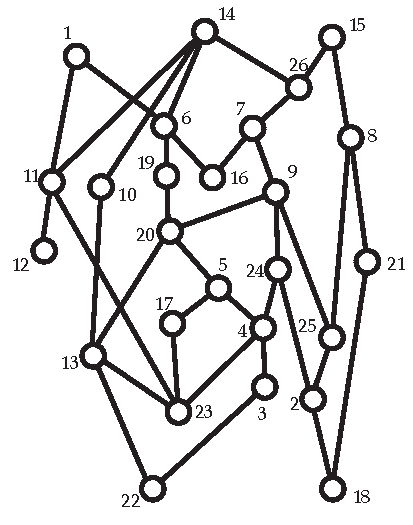
\includegraphics{posets-figs/height_ex_poset}
  \end{center}
\item For each of the two distinct (up to isomorphism) posets in 
  \autoref{fig:constructposets}, find the width $w$, an
  antichain of size $w$, and a partition of the ground set into $w$
  chains.
\item A restaurant chef has designed a new set of dishes for his
  menu. His set of dishes contains $10$ main courses, and he will
  select a subset of them to place on the menu each night. To ensure
  variety of main courses for his patrons, he wants to guarantee that
  a night's menu is neither completely contained in nor completely
  contains another night's menu. What is the largest number of menus
  he can plan using his $10$ main courses subject to this requirement?
\item Draw the diagram of the interval order represented in
  \autoref{fig:intord_to_diag_ex}.
  \begin{figure}[h]
  \begin{center}
    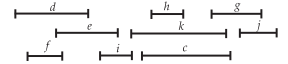
\includegraphics{posets-figs/intord_to_diag_ex}
  \end{center}
  \caption{An interval representation}\label{fig:intord_to_diag_ex}
  \end{figure}
\item Draw the diagram of the interval order represented in
  \autoref{fig:intord_to_diag_ex2}.
  \begin{figure}[h]
  \begin{center}
    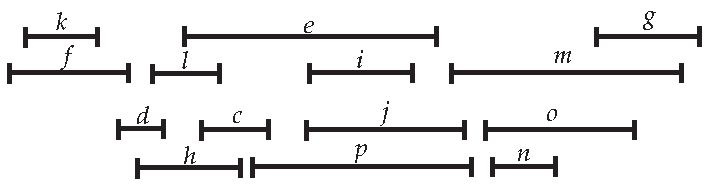
\includegraphics{posets-figs/intord_to_diag_ex2}
  \end{center}
  \caption{An interval representation}\label{fig:intord_to_diag_ex2}
  \end{figure}
\item Find an interval representation for the poset in
  \autoref{fig:intord_find_rep_ex1} or give a reason why one does not
  exist.
  \begin{figure}[h]
  \begin{center}
    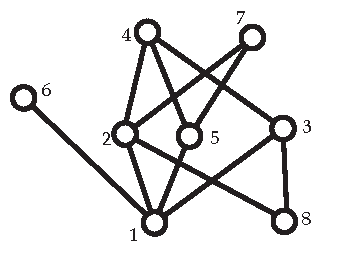
\includegraphics{posets-figs/intord_find_rep_ex1}
  \end{center}
  \caption{Is this poset an interval order?}\label{fig:intord_find_rep_ex1}
  \end{figure}
\item Find an interval representation for the poset in
  \autoref{fig:intord_find_rep_ex4} or give a reason why one does not
  exist.
  \begin{figure}[h]
  \begin{center}
    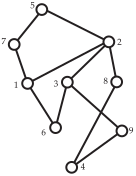
\includegraphics{posets-figs/intord_find_rep_ex4}
  \end{center}
  \caption{Is this poset an interval order?}\label{fig:intord_find_rep_ex4}
  \end{figure}
\item Find an interval representation for the poset in
  \autoref{fig:intord_find_rep_ex2} or give a reason why one does not
  exist.
  \begin{figure}[h]
  \begin{center}
    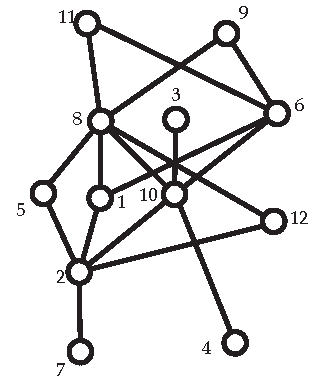
\includegraphics{posets-figs/intord_find_rep_ex2}
  \end{center}
  \caption{Is this poset an interval order?}\label{fig:intord_find_rep_ex2}
  \end{figure}
\item Find an interval representation for the poset in
  \autoref{fig:intord_find_rep_ex3} or give a reason why one does not
  exist.
  \begin{figure}[h]
  \begin{center}
    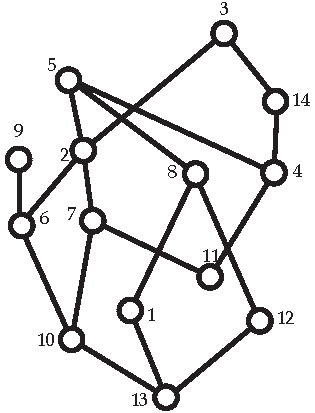
\includegraphics{posets-figs/intord_find_rep_ex3}
  \end{center}
  \caption{Is this poset an interval order?}\label{fig:intord_find_rep_ex3}
  \end{figure}
\item Use the First Fit algorithm (ordering by left endpoints) to find
  the width $w$ of the interval order shown in
  \autoref{fig:intord_firstfit_ex1} and a partition into $w$
  chains. Also give an antichain with $w$ points.
  \begin{figure}[h]
    \centering
    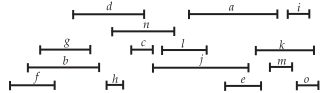
\includegraphics{posets-figs/intord_firstfit_ex1}
    \caption{An interval representation}
    \label{fig:intord_firstfit_ex1}
  \end{figure}
\item Complete the proof of Theorem\ref{thm:intord-minrep}.  \textit{Hint.}
  The key idea is to show that if $d$ is the least positive integer for
  which an interval order $\bfP$ has a representation using end points from
  $\{1,2,\dots,n\}$, then every integer $i$ from this set must be both a left
  end point and a right end point of an interval.
\item Show that every poset is isomorphic to a poset of each of the four types
  illustrated in Example~\ref{exa:construct}.  Hint: for each element $x$, choose
  some unique identifying key which is an element/prime/coordinate/observer.  Then associate
  with $x$ a structure that identifies the keys of elements from $D[x]$. 
\item The \textit{dimension} of a poset $\PXP$, denoted $\dim(\bfP)$, is the least $t$ for 
  which $P$ is the intersection of $t$ linear orders on $X$.
  \begin{enumerate}
   \item Show that the dimension of a poset $\bfP$ is the same as the dimension of its dual.
   \item Show that $\bfP$ is a subposet of $\bfQ$, then $\dim(\bfP)\le \dim(\bfQ)$.
   \item Show that the removal of a point can reduce the dimension by at most~$1$.
   \item Find the dimension of the posets in \autoref{fig:constructposets}.
   \item Use Dilworth's theorem to show that the dimension of a poset is at most its width.
   \item Use the example on the left side of \autoref{fig:FirstFit} to show that
   for every $n\ge2$, there exists a poset $\bfP_n$ on $2n$ points having width and dimension
   equal to $n$.
   \end{enumerate}
\end{enumerate}

%%% Local Variables: 
%%% mode: latex
%%% TeX-master: "book"
%%% End: 
